\documentclass{beamer}
\usepackage{geometry, amsfonts, amsmath, tikz, multicol, tikz-imagelabels, 
            multirow, pifont, xcolor, tcolorbox, soul}

\usetheme{Madrid}

\setbeamertemplate{frametitle}[default][center]
\usecolortheme{cormorant}
\title [UVA Seminar]{Search for a Self Interacting Dark Mater at the CMS Experiment }
\author[Maria Jose]{Maria Jose}
\date{\today}
\institute[UVA]{University of Virginia}
\hypersetup{
    colorlinks=true,
    linkcolor=cyan,
    filecolor=magenta,      
    urlcolor=cyan,
    pdftitle={Overleaf Example},
    pdfpagemode=FullScreen,
    }

\definecolor{uvablue}{RGB}{35,45,75}
\definecolor{uvaorange}{RGB}{229,114,0}
\definecolor{UniBlue}{RGB}{83,121,170}
\definecolor{forestgreen}{RGB}{0,128,0}
\definecolor{bronze}{rgb}{0.8, 0.5, 0.2}
\definecolor{purple}{RGB}{128,0,128}
\definecolor{maroon}{RGB}{184,15,10}
\definecolor{grey}{RGB}{128,128,128}
\definecolor{bondiblue}{rgb}{0.0, 0.58, 0.71}
\definecolor{gold}{RGB}{160,116,10}
\definecolor{peacockblue}{RGB}{0,164,180}

%\setbeamercolor{frame}{bg=black, fg =white}
%\setbeamercolor{frametitle right}{bg=gray!60!white}
%setbeamercolor{palette primary}{bg=black,fg=white}
\setbeamercolor{structure}{fg=uvaorange}
\setbeamercolor*{frametitle}{ fg =peacockblue}
\setbeamercolor*{title}{ fg = peacockblue}
%\setbeamercolor{alerted text}{fg=red!85!black}
\setbeamercolor*{palette primary}{fg =peacockblue}
\setbeamercolor*{palette secondary}{fg =peacockblue}
\setbeamercolor*{palette tertiary}{fg =peacockblue}
\setbeamercolor*{palette quaternary}{fg =peacockblue }
%\setbeamercolor*{background canvas}{bg=uvablue}
%


%\setbeamercolor*{block body}{fg=black,bg=black!10}
%\setbeamercolor*{block title alerted}{,bg=black!15}
%\setbeamercolor*{block title example}{parent(0,164,180)=example text,bg=black!15}

\imagelabelset{
coordinate label font = \sffamily\bfseries\tiny,
coordinate label distance = 1mm,
coordinate label back = black ,
coordinate label text = uvaorange,
annotation font = \normalfont\tiny,
}
\sethlcolor{black}  
%\logo{%
%  
% 
\includegraphics[width=1cm,height=1cm,keepaspectratio]{../Universitylogos/CMSlogo.png}%
%  \hspace{\dimexpr\paperwidth -2cm}%
% \vspace{\dimexpr\paperwidth }%
% 
\includegraphics[width=1cm,height=1cm,keepaspectratio]{../UniversityLogos/rotunda.jpg}%
%
%}

\begin{document}

\maketitle
\begin{frame}[t]{\textbf{Self Interacting Dark Matter Model}}
\begin{columns}
\begin{column}{.25\textwidth}
\centering
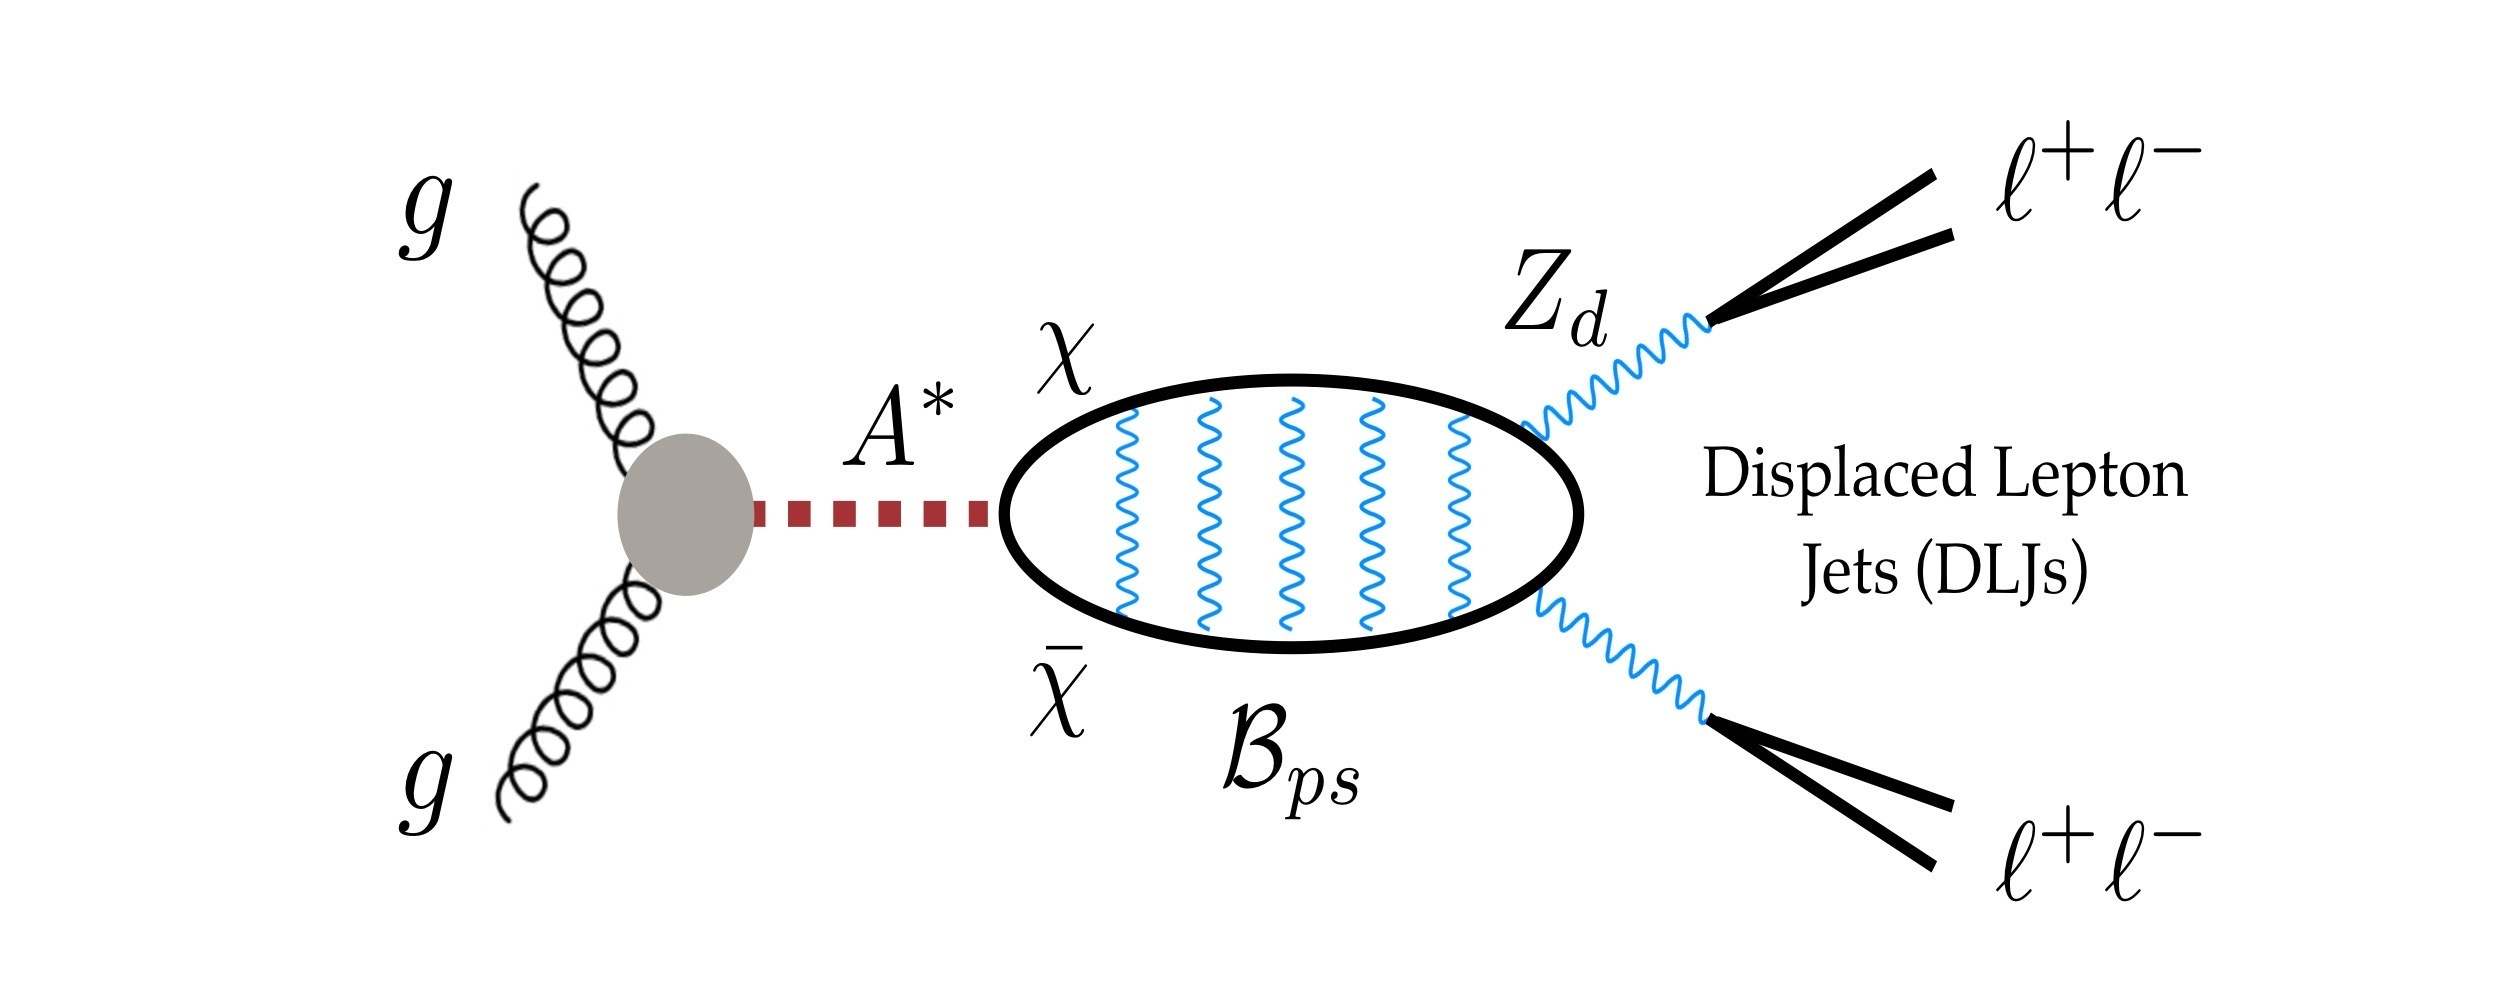
\includegraphics[width =3cm, height = 2.5 cm]{../sidm_intro_files/FeyDia.jpg}
\end{column}
\begin{column}{.5\textwidth}
\begin{enumerate}
    \item Light \textbf{$Z_d$} $\rightarrow$ \textcolor{peacockblue}{Boosted $Z_d$}
       \item Small $Z_d$ - SM Coupling \\ $\rightarrow$ \textcolor{peacockblue}{Long-Lived $Z_d$}
\end{enumerate}
\begin{tcolorbox}[colback=black,
                  colframe=uvaorange, coltext = white]

        Displaced decays of boosted $Z_d$ $\rightarrow$ \textcolor{peacockblue}{Displaced, collimated leptons }(\textcolor{uvaorange}{Displaced Lepton Jets (LJs)})
\end{tcolorbox}
    
\end{column}
\begin{column}{.25\textwidth}
\centering
\begin{annotationimage}{width=3cm, height=2.5cm}{../sidm_intro_files/lj.png}
%\draw[coordinate label  = {$Z_d \rightarrow ee$ at (0.5, -.05)}];
\draw[coordinate label  = {\textcolor{bondiblue}{LJ}  at (0.5, 0.1)}];
\draw[coordinate label  = {\textcolor{maroon}{$\mu/e$}  at (0.88, 0.9)}];
\draw[coordinate label  = {\textcolor{maroon}{$\mu/e$}  at (0.61, 0.9)}];
\end{annotationimage}
\end{column}

\end{columns}
\begin{columns}
\begin{column}{.4\textwidth}
\centering
\textbf{\textcolor{peacockblue}{Free Parameters:}}
\begin{itemize}
     \item Bound state mass ($m_B$)
     \item Dark photon mass ($m_{Z_d}$)
     \item Kinetic mixing between $Z_d$ and SM, $\epsilon$
\end{itemize}
    
\end{column}

\begin{column}{.3\textwidth}
\centering
\textbf{\textcolor{peacockblue}{Reconstruction \\
Objects:}}
\begin{itemize}
    \item PF electrons
     \item PF Photons
     \item PF Muons
     \item DSA Muons
\end{itemize}
    
\end{column}
\begin{column}{.3\textwidth}
\centering
\textbf{\textcolor{peacockblue}{Signal:}}
\begin{itemize}
    \item   $m_B$: from 100 to 1000 GeV.
     \item $m_{Z_d}$: from 0.25 to 5 GeV.
     \item $Z_d$ $L_{xy}$: from 0.3 to 300 cm.
\end{itemize}
\end{column}
\end{columns}
\end{frame}
\begin{frame}{Lepton Jets (LJs)}
\begin{itemize}
   \item Group of collimated leptons in a tight cone.
   \item We apply anti- $k_T$ clustering ($\Delta$R = 0.4) to \textbf{PF $e$, PF $\gamma$, PF $\mu$} and \textbf{DSA $\mu$}.
\end{itemize}
\begin{columns}
\begin{column}{.32\textwidth}
\textbf{\textcolor{peacockblue}{Conditions to reconstruct an LJ:}}\\
\begin{itemize}
    \item $\lvert \eta \rvert<$ 2.4
    \item $p_T>$ 30 GeV
    \item $\sum{Q_{\mu}}=$0\\
    (to prevent b-quark
    cascade decays)
\end{itemize}
\textbf{\textcolor{peacockblue}{Categories of LJs:}}\\
\begin{itemize}
    \item $e\gamma$ ($N_{\mu}=$0)
    \item $\mu$ ($N_{\mu}>=$1)
\end{itemize}
\end{column}
\begin{column}{.68\textwidth}
\begin{center}
\begin{tabular}{ |c|c|c|c|c| } 
\hline
Object Cuts & $\eta<$ & $p_T>$ & ID & Isolation\\
\hline
PF $e$& \multirow{4}{1em}{2.4}& 10 GeV &Loose& Loose\\
PF $\gamma$& & 20 GeV&Loose& Loose\\
PF $\mu$ & & 5 GeV&Loose& None\\
DSA $\mu$ & & 10 GeV& DSA& None\\
\hline


\hline
\end{tabular}
\end{center}
\textbf{\textcolor{peacockblue}{Events Categories:}}\\

\begin{itemize}
    \item $4\mu$: 2 $\mu$-type LJs
    \item $2\mu2e$: 1 $e\gamma$ -type LJ and 1 $\mu-$ type LJ
\end{itemize}
\end{column}
\end{columns}



    
\end{frame}
 \begin{frame}
    \frametitle{}
    \Huge
    Distribution Without Any Cuts
\end{frame}
\begin{frame}
   \frametitle{$Z_d \rightarrow ee$ $p_T$, $L_{xy}$ and $\Delta$R(e, e)}

   \centering
   \textcolor{uvaorange}{$m_{B}$ = 0.25 Gev, L_{xy} = 300 cm}\\
    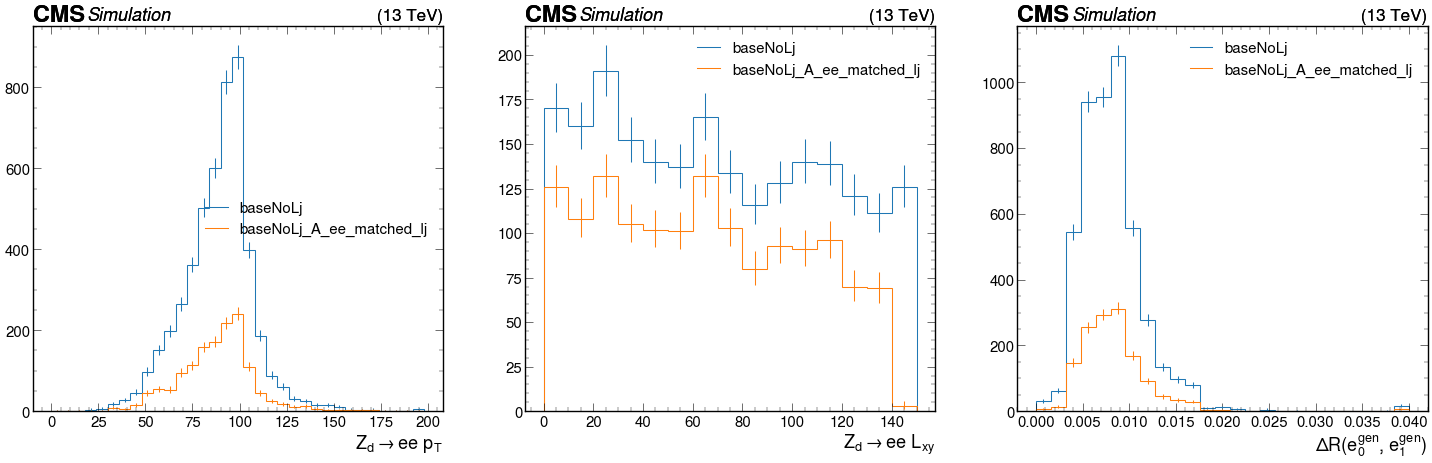
\includegraphics[width=10cm, height=2.5cm]{../sidm_files/ljRecoEffi/zd_ee_200_0p25.png}\\
    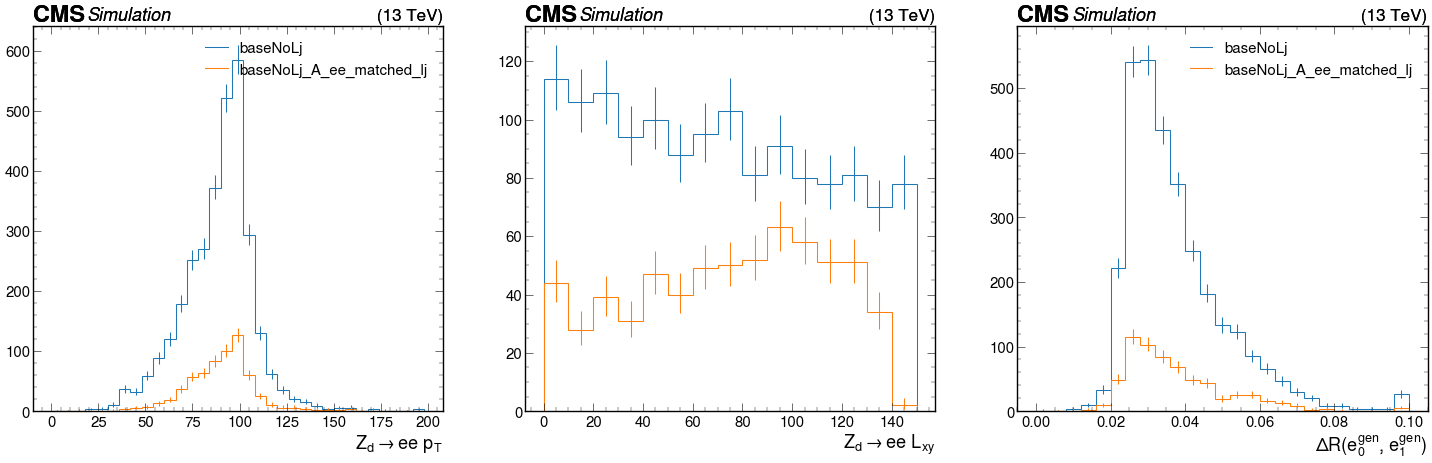
\includegraphics[width=10cm, height=2.5cm]{../sidm_files/ljRecoEffi/zd_ee_200_1p2.png}\\
    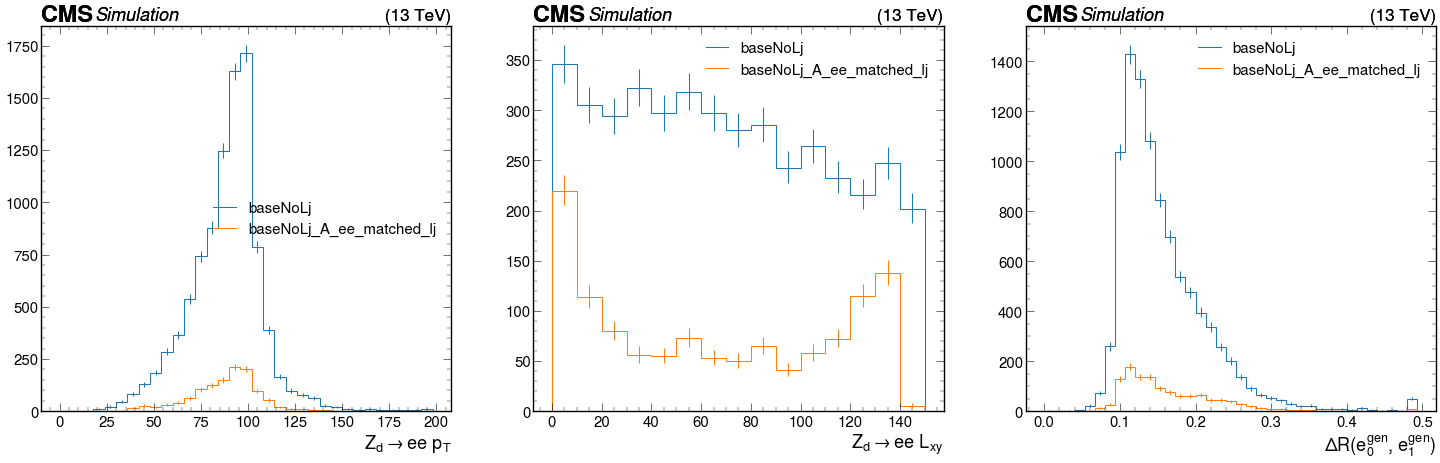
\includegraphics[width=10cm, height=2.5cm]{../sidm_files/ljRecoEffi/zd_ee_200_5.png}\\


\end{frame}
\begin{frame}
    \centering
    \Huge
    $e\gamma$ Lepton Jet Reconstruction Efficiency
\end{frame}
\begin{frame}
\frametitle{Dark Photon $p_T$}
\begin{columns}
    \begin{column}{.55\textwidth}
    \centering
    $L_{xy}<$ 150 cm\\
    \scriptsize
    \textcolor{UniBlue}{$Z_d\rightarrow ee$}, \textcolor{uvaorange}{$Z_d$ $<L_{xy}>$ = 300 cm}\\
    \textcolor{uvaorange}{$m_{Z_d}=$ 0.25 GeV (more collimated)\\}
    \begin{annotationimage}{width=3cm, height=3cm}{../sidm_files/ljRecoEffi/zd_ee_pt_200_0p25.png}
    %\draw[coordinate label  = {$Z_d \rightarrow ee$ at (0.5, -.05)}];
    %\draw[coordinate label  = {$L_{xy}<150$cm $\downarrow$  at (0.5, 1.1)}];
    \end{annotationimage}
    \begin{annotationimage}{width=3cm, height=3cm}{../sidm_files/ljRecoEffi/zd_ee_pt_1000_0p25.png}
    %\draw[coordinate label  = {\textcolor{peac}{$Z_d \rightarrow ee$} at (0.5, -0.05)}];
    %\draw[coordinate label  = {$L_{xy}<150$cm $\downarrow$ at (0.5, 1.1)}];
    \end{annotationimage}\\
    \textcolor{uvaorange}{$m_{Z_d}=$ 5 GeV (less collimated)\\}
    \begin{annotationimage}{width=3cm, height=3cm}{../sidm_files/ljRecoEffi/zd_ee_pt_200_5.png}
    \draw[coordinate label  = {\textcolor{peacockblue}{$m_{B}=$ 200 GeV} at (0.5, -.1)}];
    %\draw[coordinate label  = {$L_{xy}<150$cm $\downarrow$  at (0.5, 1.1)}];
    \end{annotationimage}
    \begin{annotationimage}{width=3cm, height=3cm}{../sidm_files/ljRecoEffi/zd_ee_pt_1000_5.png}
    \draw[coordinate label  = {\textcolor{peacockblue}{$m_B=$ 1000 GeV} at (0.5, -0.1)}];
    %\draw[coordinate label  = {$L_{xy}<150$cm $\downarrow$ at (0.5, 1.1)}];
    \end{annotationimage}
    {\tiny Note: The x ranges are different in these plots}
        
    \end{column}
    \begin{column}{.45\textwidth}
    \normalsize
    \begin{itemize}
         \item We see a sharp turn-on at 30 GeV, the cut on $p_T$ we applied on the LJs.
         \vspace{1pt}
         \item For both more collimated and less collimated the efficiency increases as a function of $p_T$ ,
         \vspace{1pt}
         \item Overall lower efficiency for the less collimated leptons.
    \end{itemize}  
    \end{column}
    \end{columns}

\end{frame}
\begin{frame}[t]{$Z_d$ $L_{xy}$}
    \centering
     $Z_d$ $p_T >$ 30 GeV\\
     \scriptsize
    \textcolor{peacockblue}{$Z_d \rightarrow ee$}, \textcolor{uvaorange}{$m_B$ = 200 GeV, $Z_d$ $<L_{xy}>$ = 300 cm}\\
    \centering
    \begin{annotationimage}{width=3cm, height=3cm}{../sidm_files/ljRecoEffi/zd_ee_lxy_200_0p25.png}
    \draw[coordinate label  = {$m_{Z_d}$ = 0.25 GeV at (0.5, -0.1)}];
    \end{annotationimage}
    \begin{annotationimage}{width=3cm, height=3cm}{../sidm_files/ljRecoEffi/zd_ee_lxy_200_1p2.png}
    \draw[coordinate label  = {$m_{Z_d}$ = 1.2 GeV at (0.5, -0.1)}];
    \end{annotationimage}
    \begin{annotationimage}{width=3cm, height=3cm}{../sidm_files/ljRecoEffi/zd_ee_lxy_200_5.png}
    \draw[coordinate label  = {$m_{Z_d}$ = 5 GeV at (0.5, -0.1)}];
    \end{annotationimage}\\
    {\tiny \vspace{-5pt}(more collimated) \hspace{5cm} (less collimated)}\\
    \normalsize
    \begin{itemize}
        \item We see good efficiency for all the regions of $L_{xy}$ for more collimated signal.
        \item As the $Z_d$ mass increases, the efficiency drops in the mid ranges of $L_{xy}
    \end{itemize}
\end{frame}
\begin{frame}[t]{$Z_d$ $L_{xy}$ in Wider Range}
    \centering
     $Z_d$ $p_T >$ 30 GeV\\
     \scriptsize
    \textcolor{peacockblue}{$Z_d \rightarrow ee$}, \textcolor{uvaorange}{$m_B$ = 200 GeV, $Z_d$ $<L_{xy}>$ = 300 cm}\\
    \centering
    \begin{annotationimage}{width=3cm, height=3cm}{../sidm_files/ljRecoEffi/e_g_effi/zd_ee_lxy_200_0p25_highRange.png}
    \draw[coordinate label  = {$m_{Z_d}$ = 0.25 GeV at (0.5, -0.1)}];
    \end{annotationimage}
    \begin{annotationimage}{width=3cm, height=3cm}{../sidm_files/ljRecoEffi/e_g_effi/zd_ee_lxy_200_1p2_highRange.png}
    \draw[coordinate label  = {$m_{Z_d}$ = 1.2 GeV at (0.5, -0.1)}];
    \end{annotationimage}
    \begin{annotationimage}{width=3cm, height=3cm}{../sidm_files/ljRecoEffi/e_g_effi/zd_ee_lxy_200_5_highRange.png}
    \draw[coordinate label  = {$m_{Z_d}$ = 5 GeV at (0.5, -0.1)}];
    \end{annotationimage}\\
    {\tiny \vspace{-5pt}(more collimated) \hspace{5cm} (less collimated)}\\
    \normalsize
    \begin{itemize}
        \item We see good efficiency for all the regions of $L_{xy}$ for more collimated signal.
        \item As the $Z_d$ mass increases, the efficiency drops in the mid ranges of $L_{xy}
    \end{itemize}
\end{frame}
\begin{frame}[t]{$Z_d$ $L_{xy}$ in 3 different categories}
    \centering
     $Z_d$ $p_T >$ 30 GeV\\
     \scriptsize
    \textcolor{UniBlue}{$Z_d \rightarrow \mu\mu$}, \textcolor{uvaorange}{$m_B$ = 200 GeV, $Z_d$ $<L_{xy}>$ = 300 cm}\\
    \centering
    \begin{annotationimage}{width=2cm, height=2cm}{../sidm_files/ljRecoEffi/e_g_effi/zd_ee_lxy_200_0p25e.png}
    \draw[coordinate label  = {$e$-type at (-.5,0.5 )}];
    \end{annotationimage}
    \begin{annotationimage}{width=2cm, height=2cm}{../sidm_files/ljRecoEffi/e_g_effi/zd_ee_lxy_200_1p2e.png}
   % \draw[coordinate label  = {$m_{Z_d}$ = 1.2 GeV at (0.5, -0.1)}];
    \end{annotationimage}
    \begin{annotationimage}{width=2cm, height=2cm}{../sidm_files/ljRecoEffi/e_g_effi/zd_ee_lxy_200_5e.png}
    %\draw[coordinate label  = {$m_{Z_d}$ = 0.25 GeV at (0.5, -0.1)}];
    \end{annotationimage}\\
    \begin{annotationimage}{width=2cm, height=2cm}{../sidm_files/ljRecoEffi/e_g_effi/zd_ee_lxy_200_0p25g.png}
    \draw[coordinate label  = {$\gamma$-type at (-.5,0.5 )}];
    %\draw[coordinate label  = {$m_{Z_d}$ = 1.2 GeV at (0.5, -0.1)}];
    \end{annotationimage}
    \begin{annotationimage}{width=2cm, height=2cm}{../sidm_files/ljRecoEffi/e_g_effi/zd_ee_lxy_200_1p2g.png}
    %\draw[coordinate label  = {$m_{Z_d}$ = 1.2 GeV at (0.5, -0.1)}];
    \end{annotationimage}
    \begin{annotationimage}{width=2cm, height=2cm}{../sidm_files/ljRecoEffi/e_g_effi/zd_ee_lxy_200_5g.png}
    %\draw[coordinate label  = {$m_{Z_d}$ = 1.2 GeV at (0.5, -0.1)}];
    \end{annotationimage}\\
    
    \begin{annotationimage}{width=2cm, height=2cm}{../sidm_files/ljRecoEffi/e_g_effi/zd_ee_lxy_200_0p25eg.png}
    \draw[coordinate label  = {$m_{Z_d}$ = 0.25 GeV at (0.5, -0.1)}];
    \draw[coordinate label  = {$e\gamma$-type at (-.5,0.5 )}];
    \end{annotationimage}
    \begin{annotationimage}{width=2cm, height=2cm}{../sidm_files/ljRecoEffi/e_g_effi/zd_ee_lxy_200_1p2eg.png}
    \draw[coordinate label  = {$m_{Z_d}$ = 1.2 GeV at (0.5, -0.1)}];
    \end{annotationimage}
    \begin{annotationimage}{width=2cm, height=2cm}{../sidm_files/ljRecoEffi/e_g_effi/zd_ee_lxy_200_5eg.png}
    \draw[coordinate label  = {$m_{Z_d}$ = 5 GeV at (0.5, -0.1)}];
    \end{annotationimage}\\
\end{frame}
\begin{frame}[t]{ $\Delta$R($e^{gen}_0, e^{gen}_1$)}
    \centering
    $Z_d$ $p_T >$ 30 GeV, $Z_d$ $L_{xy}<$ 150 cm\\
    
    \scriptsize
    \textcolor{UniBlue}{$Z_d \rightarrow ee$},
    \textcolor{uvaorange}{$m_B$ = 200 GeV, $Z_d$ $<L_{xy}>$ = 300 cm}\\
    \begin{annotationimage}{width=3cm, height=3cm}{../sidm_files/ljRecoEffi/zd_ee_deltaR_200_0p25.png}
    \draw[coordinate label  = {$m_{Z_d}$ = 0.25 GeV at (0.5, -0.1)}];
    \end{annotationimage}
    \begin{annotationimage}{width=3cm, height=3cm}{../sidm_files/ljRecoEffi/zd_ee_deltaR_200_1p2.png}
    \draw[coordinate label  = {$m_{Z_d}$ = 1.2 GeV at (0.5, -0.1)}];
    \end{annotationimage}
    \begin{annotationimage}{width=3cm, height=3cm}{../sidm_files/ljRecoEffi/zd_ee_deltaR_200_5.png}
    \draw[coordinate label  = {$m_{Z_d}$ = 5 GeV at (0.5, -0.1)}];
    \end{annotationimage}\\
    {\tiny \vspace{-5pt}(more collimated) \hspace{5cm} (less collimated)}\\
    \normalsize
    \begin{itemize}
        \item We see non-zero efficiency in the whole range of $\Delta$R.
         \vspace{1pt}
        \item Efficiency is not changing much as a function of $\Delta$R.
         \vspace{1pt}
        \item As the $Z_d$ mass increases, overall efficiency lowers. This could be the effect of collimation.
    \end{itemize}
    {\scriptsize Note: The x ranges are different in these plots}
    
    
\end{frame}
\begin{frame}{}
        \centering
        \Huge
        $\mu$ Lepton Jet Reconstruction Efficiency
        \end{frame}

\begin{frame}[t]{$Z_d$ $p_T$}

\begin{columns}
\begin{column}{.55\textwidth}
\centering
$L_{xy}<$ 250 cm\\
\scriptsize
\textcolor{UniBlue}{$Z_d\rightarrow \mu\mu$}, \textcolor{uvaorange}{$Z_d$ $<L_{xy}>$ = 300 cm}\\
\textcolor{uvaorange}{$m_{Z_d}=$ 0.25 GeV (more collimated)\\}
\begin{annotationimage}{width=3cm, height=3cm}{../sidm_files/ljRecoEffi/zd_mumu_pt_200_0p25.png}
%\draw[coordinate label  = {$Z_d \rightarrow ee$ at (0.5, -.05)}];
%\draw[coordinate label  = {$L_{xy}<150$cm $\downarrow$  at (0.5, 1.1)}];
\end{annotationimage}
\begin{annotationimage}{width=3cm, height=3cm}{../sidm_files/ljRecoEffi/zd_mumu_pt_1000_0p25.png}
%\draw[coordinate label  = {\textcolor{UniBlue}{$Z_d \rightarrow ee$} at (0.5, -0.05)}];
%\draw[coordinate label  = {$L_{xy}<150$cm $\downarrow$ at (0.5, 1.1)}];
\end{annotationimage}\\
\textcolor{uvaorange}{$m_{Z_d}=$ 5 GeV (less collimated)\\}
\begin{annotationimage}{width=3cm, height=3cm}{../sidm_files/ljRecoEffi/zd_mumu_pt_200_5.png}
\draw[coordinate label  = {\textcolor{peacockblue}{$m_{B}=$ 200 GeV} at (0.5, -.075)}];
%\draw[coordinate label  = {$L_{xy}<150$cm $\downarrow$  at (0.5, 1.1)}];
\end{annotationimage}
\begin{annotationimage}{width=3cm, height=3cm}{../sidm_files/ljRecoEffi/zd_mumu_pt_1000_5.png}
\draw[coordinate label  = {\textcolor{peacockblue}{$m_B=$ 1000 GeV} at (0.5, -0.075)}];
%\draw[coordinate label  = {$L_{xy}<150$cm $\downarrow$ at (0.5, 1.1)}];
\end{annotationimage}
{\tiny Note: The x ranges are different in these plots}

    
\end{column}
\begin{column}{.45\textwidth}
\normalsize
\begin{itemize}
  \item We see a sharp turn-on at 30 GeV, the cut on $p_T$ we applied on the LJs.
     \vspace{1pt}
  \item After the turn-on, efficiency slightly decreases as the $p_T$ increases for both cases.
     \vspace{1pt}
\item Efficiency decreases as a funtion of $p_T$ for more collimated signal.
\item Effiency is more or less constant for less collimated signal.
\end{itemize}  
\end{column}
\end{columns}
\end{frame}
\begin{frame}[t]{$Z_d$ $L_{xy}$}
    \centering
    $Z_d$ $p_T >$ 30 GeV\\
     \scriptsize
\textcolor{UniBlue}{$Z_d \rightarrow \mu\mu$}, \textcolor{uvaorange}{$m_B$ = 200 GeV, $Z_d$ $<L_{xy}>$ = 300 cm}\\
\centering
\begin{annotationimage}{width=3cm, height=3cm}{../sidm_files/ljRecoEffi/zd_mumu_lxy_200_0p25.png}
    \draw[coordinate label  = {$m_{Z_d}$ = 0.25 GeV at (0.5, -0.2)}];
    \end{annotationimage}
    \begin{annotationimage}{width=3cm, height=3cm}{../sidm_files/ljRecoEffi/zd_mumu_lxy_200_1p2.png}
    \draw[coordinate label  = {$m_{Z_d}$ = 1.2 GeV at (0.5, -0.2)}];
    \end{annotationimage}
    \begin{annotationimage}{width=3cm, height=3cm}{../sidm_files/ljRecoEffi/zd_mumu_lxy_200_5.png}
    \draw[coordinate label  = {$m_{Z_d}$ = 5 GeV at (0.5, -0.2)}];
    \end{annotationimage}\\
{\tiny \vspace{-9pt}(more collimated) \hspace{5cm} (less collimated)}\\
\normalsize
\begin{itemize}
    \item Similar behaviour for all three $Z_d$ masses.
     \item Very low efficiency in the DSA muon regions.
\end{itemize}

\end{frame}
\begin{frame}[t]{$Z_d$ $L_{xy}$ in 3 different categories}
 \centering
 $Z_d$ $p_T >$ 30 GeV\\
 \scriptsize
 \textcolor{UniBlue}{$Z_d \rightarrow \mu\mu$}, \textcolor{uvaorange}{$m_B$ = 200 GeV, $Z_d$ $<L_{xy}>$ = 300 cm}\\
 \centering
 \begin{annotationimage}{width=2cm, height=2cm}{../sidm_files/ljRecoEffi/pf_dsa_effi/zd_mumu_lxy_200_0p25pf.png}
 \draw[coordinate label  = {$PF$-type at (-.5,0.5 )}];
 \end{annotationimage}
 \begin{annotationimage}{width=2cm, height=2cm}{../sidm_files/ljRecoEffi/pf_dsa_effi/zd_mumu_lxy_200_1p2pf.png}
 % \draw[coordinate label  = {$m_{Z_d}$ = 1.2 GeV at (0.5, -0.1)}];
 \end{annotationimage}
 \begin{annotationimage}{width=2cm, height=2cm}{../sidm_files/ljRecoEffi/pf_dsa_effi/zd_mumu_lxy_200_5pf.png}
  %\draw[coordinate label  = {$m_{Z_d}$ = 0.25 GeV at (0.5, -0.1)}];
  \end{annotationimage}\\
  \begin{annotationimage}{width=2cm, height=2cm}{../sidm_files/ljRecoEffi/pf_dsa_effi/zd_mumu_lxy_200_0p25dsa.png}
  \draw[coordinate label  = {$DSA$-type at (-.5,0.5 )}];
  %\draw[coordinate label  = {$m_{Z_d}$ = 1.2 GeV at (0.5, -0.1)}];
  \end{annotationimage}
  \begin{annotationimage}{width=2cm, height=2cm}{../sidm_files/ljRecoEffi/pf_dsa_effi/zd_mumu_lxy_200_1p2dsa.png}
  %\draw[coordinate label  = {$m_{Z_d}$ = 1.2 GeV at (0.5, -0.1)}];
  \end{annotationimage}
  \begin{annotationimage}{width=2cm, height=2cm}{../sidm_files/ljRecoEffi//pf_dsa_effi/zd_mumu_lxy_200_1p2dsa.png}
  %\draw[coordinate label  = {$m_{Z_d}$ = 1.2 GeV at (0.5, -0.1)}];
  \end{annotationimage}\\
  
  \begin{annotationimage}{width=2cm, height=2cm}{../sidm_files/ljRecoEffi/pf_dsa_effi/zd_mumu_lxy_200_0p25pfdsa.png}
  \draw[coordinate label  = {$m_{Z_d}$ = 0.25 GeV at (0.5, -0.1)}];
  \draw[coordinate label  = {$PF-DSA$-type at (-.5,0.5 )}];
  \end{annotationimage}
  \begin{annotationimage}{width=2cm, height=2cm}{../sidm_files/ljRecoEffi/pf_dsa_effi/zd_mumu_lxy_200_1p2pfdsa.png}
  \draw[coordinate label  = {$m_{Z_d}$ = 1.2 GeV at (0.5, -0.1)}];
  \end{annotationimage}
  \begin{annotationimage}{width=2cm, height=2cm}{../sidm_files/ljRecoEffi/pf_dsa_effi/zd_mumu_lxy_200_5pfdsa.png}
  \draw[coordinate label  = {$m_{Z_d}$ = 5 GeV at (0.5, -0.1)}];
  \end{annotationimage}\\
 \end{frame}
 \begin{frame}[t]{ $\Delta$R($\mu^{gen}_0, \mu^{gen}_1$)}
 \centering
 $Z_d$ $p_T >$ 30 GeV, $Z_d$ $L_{xy}<$ 250 cm\\
 \scriptsize
 \textcolor{UniBlue}{$Z_d \rightarrow \mu\mu$},
 \textcolor{uvaorange}{$m_B$ = 200 GeV, $Z_d$ $<L_{xy}>$ = 300 cm}\\
 \begin{annotationimage}{width=3cm, height=3cm}{../sidm_files/ljRecoEffi/zd_mumu_deltaR_200_0p25.png}
\draw[coordinate label  = {$m_{Z_d}$ = 0.25 GeV at (0.5, -0.05)}];
\end{annotationimage}
\begin{annotationimage}{width=3cm, height=3cm}{../sidm_files/ljRecoEffi/zd_mumu_deltaR_200_1p2.png}
\draw[coordinate label  = {$m_{Z_d}$ = 1.2 GeV at (0.5, -0.05)}];
\end{annotationimage}
\begin{annotationimage}{width=3cm, height=3cm}{../sidm_files/ljRecoEffi/zd_mumu_deltaR_200_5.png}
\draw[coordinate label  = {$m_{Z_d}$ = 5 GeV at (0.5, -0.05)}];
\end{annotationimage}\\
{\tiny \vspace{-8pt}(more collimated) \hspace{5cm} (less collimated)}\\
\normalsize
\begin{itemize}
    \item Effiency is not varying as function of $\Delta$R. 
     \vspace{1pt}

\end{itemize}
{\scriptsize Note: The x ranges are different in these plots}


\end{frame}
\begin{frame}
\frametitle{}
\end{frame}
\end{document}
